\documentclass{article}
\title{Twiddle -- A DSL for the Functional Bit-hacker}
\author{Michael Buch}

\usepackage[inline]{enumitem} % inline numbered lists
\usepackage[left=2cm,right=2cm]{geometry}
\usepackage{verbatim} % for comments
\usepackage{graphicx}
\usepackage{listings}
\usepackage{color}

\definecolor{dkgreen}{rgb}{0,0.6,0}
\definecolor{gray}{rgb}{0.5,0.5,0.5}
\definecolor{mauve}{rgb}{0.58,0,0.82}
\lstset{frame=tb,
  aboveskip=3mm,
  belowskip=3mm,
  showstringspaces=false,
  columns=flexible,
  basicstyle={\small\ttfamily},
  numbers=none,
  numberstyle=\tiny\color{gray},
  keywordstyle=\color{blue},
  commentstyle=\color{dkgreen},
  stringstyle=\color{mauve},
  breaklines=true,
  breakatwhitespace=true,
  tabsize=3
}

\begin{document}
\maketitle
\frenchspacing

\begin{abstract}
It is useful (and fun!) to bit twiddle i.e. perform arithmetic and manipulate data at the granularity of individual bits. Traditionally there is a compromise one has to make between using a low-level unsafe language that allows bit-twiddling versus a safe high-level language in which the type system or language design prohibit operations at bit-level (without additional complexity). The \textit{Twiddle} domain-specific language (DSL) is an embedded language written in Scala that generates bit-twiddling style C code. The language offers several modes of operation, useful for quick prototyping, debugging and custom extensions:
\begin{enumerate*}[label=(\arabic*)]
	\item Tracing interpreter
	\item Scala evaluator
	\item Twiddle AST generator
	\item C code generator
\end{enumerate*}.
Thus our language is a tool for the curious, a tool for safe bit-hackers and a tool for someone looking to get a bit more performance out of his high-level language.
\end{abstract}

\section{Motivation}
No need to worry about syntax such as semicolons, operator precedence, asterisk locations or qualifier usages.
Bithacks in \cite{anderson2005bit} have been verified
\section{The Language \& Architecture}
\begin{figure}[t]
	\centering
	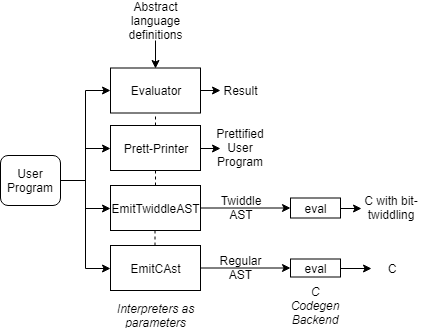
\includegraphics[scale=1]{twiddle_arch.png}
	\caption{Architecture of the Twiddle framework}\label{twiddle_arch}
\end{figure}
\subsection{Core}
The core of the language is split into modular pieces of functionality implemented as traits. As is common practice with tagless final interpreters (see section \ref{subsec:tagless}) we parameterize each set of language features with an evaluator that describes how each feature within its context. Below we briefly describe some of the core feature set which are implemented as traits in \textbf{core.scala}:
\begin{itemize}
	\item \textbf{Nums}: Defines abstract interpretation of numeric Scala types including \texttt{Int, Double, Float}. It is generic over the type of input number supplied. Operations involving numeric types in the core language thus have to also be generic over numeric types. This is fine for integral numbers but gets problematic for fractional operations such as division.
	\item \textbf{Arithmetic}: Basic mathematical operations that operate on the interpretation of core's \texttt{num}. Some operations are generic over the input type while others are explicitly for fractional versus integral types.
	\item \textbf{Bools}: Includes both the interpretation of Scala's \texttt{Boolean} type and also of constructs operating on said booleans such as if-statements, ternary operators and logical operators.
	\item \textbf{Lambda}: Interpretation of lambda definition and application. Scala's lambda maps cleanly to the concept of a lambda in the lisp-like user-level language. However, a mapping to C is less straightforward and described in section \ref{subsec:ast_interpreter}
	\item \textbf{LispLike}: Contains a limited set of Lisp primitives to be able to create lists using \texttt{cons/car/cdr}. A \texttt{begin} primitive was added mainly as a way to collect the AST nodes created in a code snippet when interpreting using \texttt{EmitTwiddleAST} since without it Scala would simply return the last generated statement. Essentially it is a wrapper around a Scala \texttt{List}.
\end{itemize}

The traits prefixed with a ``C'' such as the following ones listed are the operations taken from Anderson's set of bithacks\cite{anderson2005bit}.
\begin{itemize}
	\item \textbf{CMathOps}: Mathematical operations that when passed to the codegeneration backend produce bit-twiddled implementations. Typically in other languages these would correspond to standard library functions such as \textbf{scala.math.log10} for \texttt{log10}.
	\item \textbf{Bits}: Includes definitions of the \texttt{bits} term, which is simply the interpretation of a numeric type, and functions whose goal is to operate on the structure of bit patterns of an integer such as reversing bit sequences.
\end{itemize}

\subsection{Evaluators}
Each term in the language is a function whose parameters and return type are wrapped in the abstract type of the interpreter that is evaluating the function. The second column of figure \ref{twiddle_arch} shows the current set of supported interpreters.

\textit{Evaluator} corresponds to the \texttt{implicit object Eval} in \textbf{interpreter.scala}. Here terms are evaluated and returned as values in the host language (i.e. Scala).

\textit{Pretty-Printer} corresponds to the \texttt{implicit object Show} in \textbf{interpreter.scala}. Here all terms are of type \texttt{String} and evaluation of a term yields its pretty-printed version.

\textit{EmitTwiddleAST} corresponds to the Scala object of the same name in \textbf{codegen.scala}. This is the core of the Twiddle code generator.

\section{Codegen}
\subsection{Twiddle AST}
The code generation part of the Twiddle framework is shown in the bottom two branches of the flow chart in figure \ref{twiddle_arch}. As a way to map modularly and extensibly between a high-level language like the lambda calculus variant in our case to a low-level language like C we introduced a intermediate representation (IR) of the user-level Twiddle code structured as an abstract syntax tree (AST). The IR language includes features that would not fit to the semantics of the high-level language but are needed for bit-twiddling or general operations in C. Nodes in the AST are all represented by the \texttt{abstract trait Term} and evaluation of the terms occurs on nested tuples of terms (i.e. \texttt{Tup(Term, Tup(Tup(Term, Term)...)...)}) to be able to conveniently manipulate it from within the evaluator of the AST. Where there is only a small set of one-to-one mappings between terms in the object language and actual C language constructs, the IR mimics a subset of valid terms in C. Figure DIAGRAM NEEDED shows valid terms in the Twiddle IR. Distinction between primitives, expressions, C language identifiers, etc. is not provided since our evaluators on the AST did not require it. The term types can, however, be refined with additional traits if one needs to special-case according to certain classes of C language features.

\subsubsection{Builtins}
There is no distinction between language features and built-in functions in Twiddle. Every language feature is a function that describes its evaluation in the interpreter context. We implement common operations in the associated traits and inject it into the abstract \texttt{Exp[T[\_]]} trait. These operations have been chosen with bit-twiddling in mind. More often than not there is a corresponding algorithm using bithacks CITATION NEEDED which the codegen back-end implements in the IR.

We considered several ways of supporting bit-twiddling operations. In the final version of Twiddle we have a specific bit-twiddling backend whose sole purpose is to translate arithmetic, string or bit operations, provided as language features, into equivalent bithacks CITATION NEEDED. While a step in the right direction, an alternative (or extension) would be to detect certain user patterns or even annotations in the source, and map the patterns into bithack patterns. An example could be the reversal of a string. If currently a user is not aware of the Twiddle provided builtin \texttt{reverse(s: T[String])}, a user might choose to implement his own reversal algorithm and Twiddle would simply generate plain C. A more advanced backend detects these patterns from the AST.

\subsubsection{Bits}
So far we have only discussed mathematical or string operations that utilize arithmetic or logical shift operators to achieve a task that would have required control flow constructs in a naive implementation. The term bit-twiddling, however, also encompasses operations directly on the bit representation of terms. For this purpose, we implemented the \texttt{bits(a: T[Int]): T[BitSet])} term in the core language. As the function definition implies, an evaluation of \texttt{bits} will turn an integer into a logical representation of bits. We say logical representation because this translation is different between the Twiddle front-end evaluators and the codegen IR. In the Twiddle AST bits are simply represented as integers. Operations on said integers that would in the C layer operate on bits are responsible for declaring the necessary integers as \texttt{unsigned long}. In the front-end evaluator, however, a conversion does take place from integer to a Scala BitSet.

\subsubsection{Other Useful Constructs}
As implied above, not all IR terms are features in the core language, thus terms such as \texttt{Ref(e: Term)} or \texttt{Assign(v: Term, e: Term)} are helper terms used to ease the transition from user-level language to C.
Variable declarations and assignment

\subsection{Twiddle AST Interpreters}\label{subsec:ast_interpreter}
A consequence of the Tagless style of the core language is that in order to achieve a generic expression type that is used across all interpreters and be able to interpret the same piece of code in multiple ways, we need to implement language features across several interpreters that are semantically sound. For the \texttt{EmitTwiddleAST} interpreter this poses a challenge since some of the functional higher-level constructs do not map cleanly onto C-style programs. A prime example is the lambda/apply pair. A way to map lambdas to C is to convert the lambda into a function definition, storing the function body together with a unique function name in the internal interpreter state, return the function name to the user and on applications of the function name generate a C function call. For this purpose we implemented term \texttt{Func( FILL )} and \texttt{App( FILL )}. However, retrieving the function body requires intrusive changes around several components of the framework and is left as an open exercise for future versions. Currently a \texttt{lam} returns a closure to the user which he is responsible for applying i.e. passing to \texttt{app} which then evaluates the lambda.

\subsubsection{Auxiliary Machinery}
To avoid name clashes we use a file-static counter that increments whenever a call to \texttt{gensym} is performed.

In procedural languages one has to be able to assign an expression to a variable to track state and perform any kind of meaningful computation. This is problematic in our ``greedy-print'' model of code generation since we can generate syntactically invalid expression assignments. An example would be generating code from:
\begin{lstlisting}[language=Scala]
val x = 5
val y = add10(x)
val z = 2 * y
\end{lstlisting}
\begin{lstlisting}[language=C]
int z = 2 * int x = 5; + 10 // Syntax error
\end{lstlisting} Since we do not perform constant propagation or evaluation of terms prior to emitting Twiddle source, we need a mechanism to signal that an expression returns a meaningful result and a subsequent expression should use that value instead. Taking inspiration from Let-insertion in ANF-conversion of functional languages, we introduced a \texttt{Result(v: Var, t: Term)} into the IR that will assign the result of evaluating some expression $t$ to the variable $v$ in the generated code.

Funcdefs
Gensym
Return helper
IO
Ensuring correct syntax
\section{Design Choices}
\subsection{Language Embedding}
\subsection{Scala}
\subsection{Tagless Final Style}\label{subsec:tagless}
\section{Conclusion \& Future Work}
\begin{itemize}
	\item Benefits of shallow embeddings. Can fall back to scala features. Don't need to implement side effects in object language necessarily.
	\item Extend LMS
	\item Use tagless evaluator for AST evaluation
	\item Writing larger programs
	\item Other backends
\end{itemize}

\bibliographystyle{ieeetran}
\bibliography{twiddle}
\end{document}